\documentclass[a4paper,12pt]{report} % format a4, taille du texte, type de document
\usepackage[utf8]{inputenc} % afficher les accents correctement
\usepackage[T1]{fontenc} % police contenant caractères spéciaux français
\usepackage[francais]{babel} % langue du texte
\usepackage[colorlinks=true]{hyperref} % activer les liens hypertextes
\usepackage{graphicx} % importer les images
\usepackage{phdthesis}  %templte utilisé
\usepackage[hcentering,textwidth=150mm,textheight=225mm]{geometry} %marges
\usepackage[Bjornstrup]{fncychap} %affiche les chapitres differement
\usepackage{tocloft} %affichage different pour la table des marères
\usepackage{caption} 
\usepackage{lipsum}
\usepackage{listings}
\usepackage{color}

\cfoot{\thepage}

%\rhead{Rapport de stage ST50}
\lfoot{\textbf{UTBM ST50}}
\cfoot{}

\setcounter{secnumdepth}{3}

\renewcommand{\cfttoctitlefont}{\center\large\bfseries\MakeUppercase} % change toc title to upper case

\hypersetup{
  colorlinks,
  linkcolor=wine-stain,
  linktoc=all
}

\definecolor{dkgreen}{rgb}{0,0.6,0}
\definecolor{gray}{rgb}{0.5,0.5,0.5}
\definecolor{mauve}{rgb}{0.58,0,0.82}

\lstdefinestyle{custompython}{frame=tb,
  language=Python,
  aboveskip=3mm,
  belowskip=3mm,
  showstringspaces=false,
  columns=flexible,
  basicstyle={\small\ttfamily},
  numbers=none,
  numberstyle=\tiny\color{gray},
  keywordstyle=\color{blue},
  commentstyle=\color{dkgreen},
  stringstyle=\color{mauve},
  breaklines=true,
  breakatwhitespace=true,
  tabsize=3
}

\lstdefinestyle{customruby}{frame=tb,
  language=Ruby,
  aboveskip=3mm,
  belowskip=3mm,
  showstringspaces=false,
  columns=flexible,
  basicstyle={\small\ttfamily},
  numbers=none,
  numberstyle=\tiny\color{gray},
  keywordstyle=\color{blue},
  commentstyle=\color{dkgreen},
  stringstyle=\color{mauve},
  breaklines=true,
  breakatwhitespace=true,
  tabsize=3
}

\definecolor{Darkblue}{rgb}{0,0,0.4}
\definecolor{wine-stain}{rgb}{0.5,0,0}

\begin{document}


\tableofcontents
%!TEX root =/Users/ludovicl/Dropbox/Cours/UTBM/P15/RapportStage/main.tex


\chapter{Présentation de l'entreprise}


Tech4Team est une startup fondée en juillet 2013 par deux entrepreneurs. Elle propose aujourd'hui deux produits majeurs Inventor-e et Arenametrix.

\section{Inventor-e}
Inventor-e est un logiciel de gestion de planning, de suivi d’états des lieux et de pilotage de maintenance. Il est conçu pour les infrastructures sportives et culturelles multifonctions.

Le logiciel fonctionne sur le principe de client-serveur. L'utilisateur utilise une tablette Android pour faire un état des lieux ou visualiser son planning. Les photos et autres données sont ensuite synchronisées dans une base de données sur un serveur distant. Il est alors possible pour l'utilisateur de visualiser les informations depuis un portail web.

\begin{center}
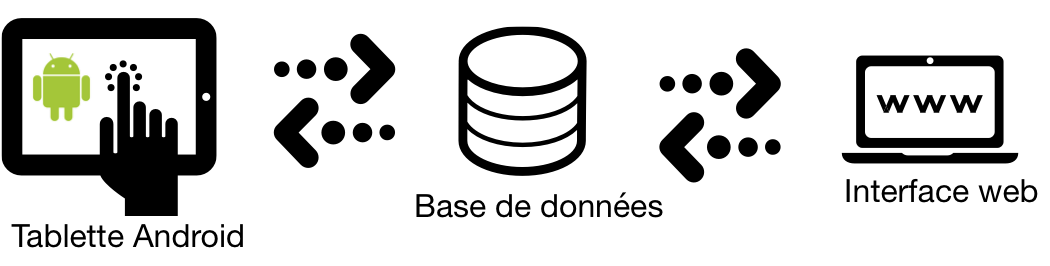
\includegraphics[scale=0.7]{images/inventore.png}
\captionof{figure}{Principe de fonctionnement d'inventor-e}
\label{inventore}
\end{center}

D'une manière plus technique l'application est développée pour Android 4.0 ou ultérieur, la base de données utilise PostegreSQL et l'interface web est développée avec le framework Ruby on Rails.

\section{Arenametrix}
Arenametrix est une solution logicielle, flexible, clé en main et intégrée de Big Data (analyse et exploitation des données billetteries), disponible en SaaS, pour la connaissance et la fidélisation des publics, la prospection ciblée et la mise en place d'une nouvelle politique de tarification

Arenametrix de décompose en trois briques technologiques indépendantes ou combinées : 
\begin{itemize}
  \item[\textbullet] Arena-public : Socle e-CRM
  \item[\textbullet] Arena-prospection : Prospection ciblée
  \item[\textbullet] Arena-pricing : Tarification dynamique
\end{itemize}

\begin{center}
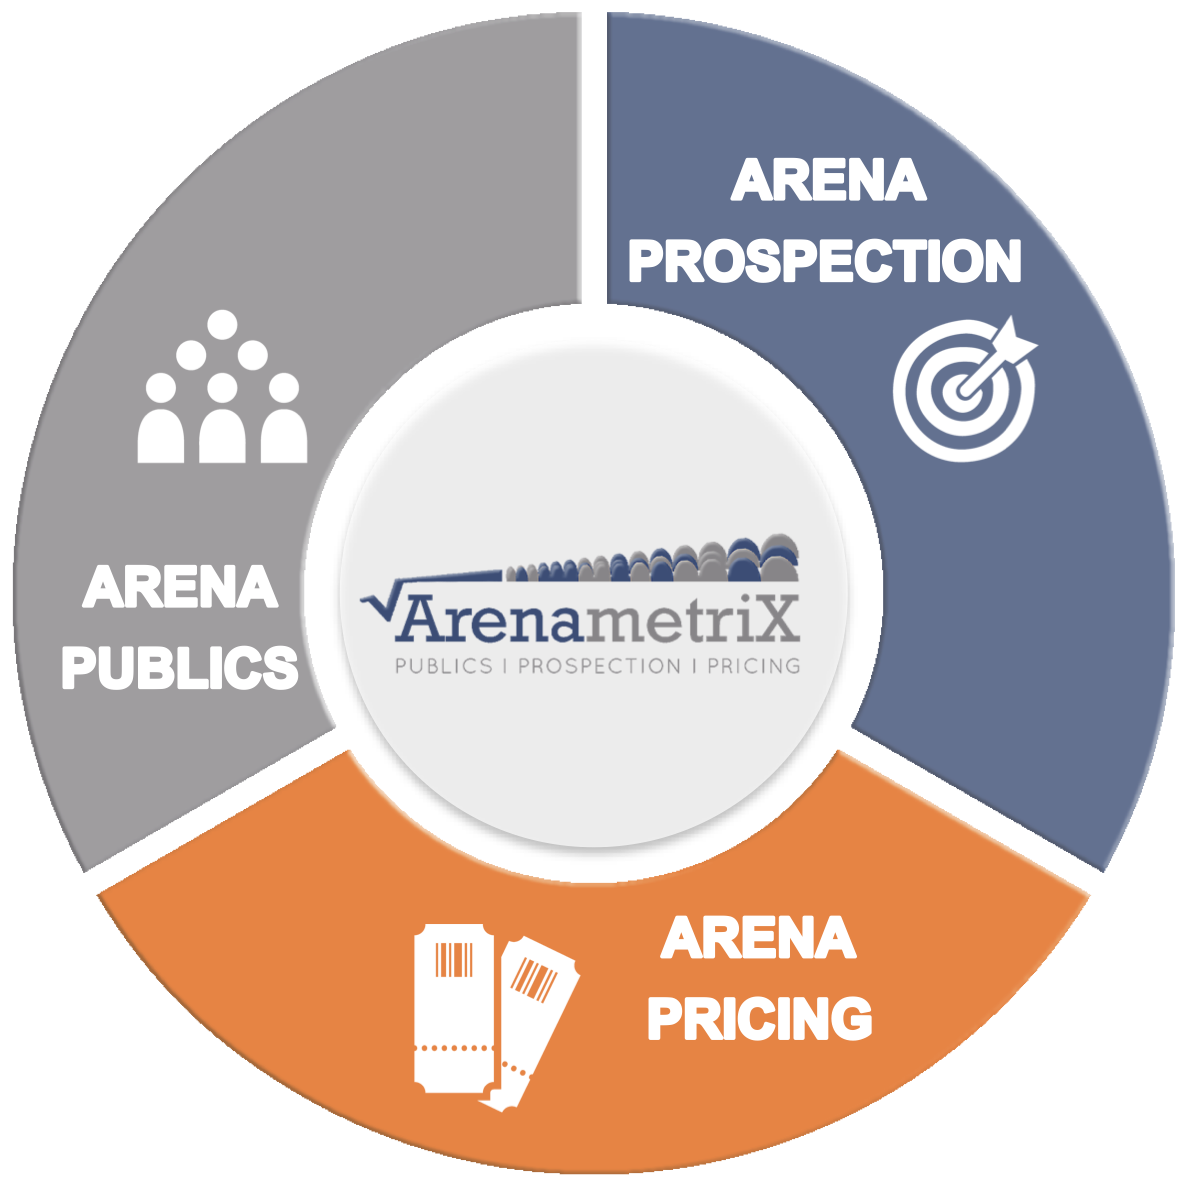
\includegraphics[scale=0.45]{images/arenametrix.png}
\captionof{figure}{Vision à 360\ensuremath{^\circ}  de Arenametrix}
\label{arenametrix}
\end{center}

\subsection{Arena-public}
Arena-public est le socle e-CRM d’exploitation des données publics.

Il permet :
\begin{itemize}
  \item[\textbullet] La centralisation des données publics, B to B et B to C
  \item[\textbullet] Le nettoyage et enrichissement des données (sexe, âge, lieu de résidence, fréquentation du stade, dépenses merchandising…)
  \item[\textbullet] La visualisation graphique de la base de données à 360\ensuremath{^\circ}
  \item[\textbullet] L'analyse mono-variable et bi-variable en croisant des données identitaires et de consommation
\end{itemize}

\subsection{Arena-prospection}
Module d’optimisation du démarchage commercial.

Ce module permet :
\begin{itemize}
  \item[\textbullet] La sélection d’une liste de contacts
  \item[\textbullet] Le classement des prospects selon leur probabilité de souscription
  \item[\textbullet] La gestion interfacée d’une campagne de téléprospection, de mailing et de SMS auprès des prospects
  \item[\textbullet] L'analyse des retours : réaction au démarchage, taux de conversion et intégration à la priorisation
\end{itemize}

\subsection{Arena-pricing}
Module de yield management.

Ce module permet :
\begin{itemize}
  \item[\textbullet] La création de typologies de publics par segmentation et profilage
  \item[\textbullet] La prévision de la demande en billets pour un événement
  \item[\textbullet] Recommandations tarifaires en fonction de la date et de la catégorie
  \item[\textbullet] La gestion des flux par le prix, en transparence avec le client final
\end{itemize}

\subsection{Objectifs}
Tech4Team prévoir plusieurs objectifs pour son produit :
\begin{itemize}
	\item[\textbullet] Démocratisation de l'accès à la culutre en ouvrant la voie à des prix différenciés
	\item[\textbullet] Stabilisation voir hausse de la rentabilité des structures culturelles en augmentant le chiffre d'affaires billereterie de 5 à 7\%
\end{itemize}

\section{Fonctionnement de l'entreprise et répartition des tâches}
Durant la majeure partie de mon stage l'équipe se composé de six stagiaires, cinq en développement et un commercial, un développeur expérimenté en cdi et les deux fondateurs. \\

Sur Arenametrix : 
\begin{itemize}
  \item[\textbullet] Un stagiaire s'occupait du front-end et de l'affichage des données
  \item[\textbullet] Un stagiaire s'occupait de la partie analyse de données
  \item[\textbullet] Un stagiaire s'occupait du scoring
  \item[\textbullet] Le développeur en cdi validait nos choix techniques sur le produit et jouait également le rôle d'administrateur système
  \item[\textbullet]Moi, je m'occupais du back-end et de l'importation des données
\end{itemize} \

Sur Inventor-e : 
\begin{itemize}
  \item[\textbullet] Un stagiaire s'occupait de l'application Android
  \item[\textbullet] Le développeur en cdi s'occupait de la base de données et de l'interface web
\end{itemize}

\leavevmode
\\
Les deux fondateurs s'occupaient des relations clients avec le commercial et nous attribuaient des tâches pour améliorer et faire évoluer les produits. Des réunions sont réguliérmeents organisés pour définir les architecture logiciels, de base de données et les moyens techniques à utiliser. 
\\ \\
La gestion de projets se fait avec l'outil open source Redmine. Pour la gestion du code source, nous utilisons Git et la plateforme Gitlab.


%!TEX root =/Users/ludovicl/Dropbox/Cours/UTBM/P15/RapportStage/main.tex
\chapter{Mise en situation et activités effectuées}

Lors de mon entretien de stage les fondateurs de l'entreprise m'ont indiqué que j'allais utiliser les technologies Ruby et Python. Le sujet était donc de travailler avec le CTO sur la base de données et de coder le back-end de l'importation de données billetteries.
\\ 

À mon arrivée l'architecture d'une base de données était déjà réalisée. Mais elle n'était pas utilisée et encore moins remplie. J'ai donc du rapidement l'adapter en fonction des premières données billetteries que j'ai reçue et que je devais insérer. Plusieurs stagiaires avaient géré la base de données auparavant, certaines tables étaient redondantes (parfois en français et en anglais), certaines autres ne contenaient pas de clés étrangères (juste l'id d'une autre table). J'ai donc au fur et à mesure corrigé tout ça.


\section{Importation manuel de données billetteries des clients dans ArenaPricing}

L'une de mes premières tâches en arrivant dans l'entreprise est de créer un logiciel permettant à Tech4Team et à certains clients de facilement insérer dans notre base de données un fichier CSV\footnote{Comma-separated values, connu sous le sigle CSV, est un format informatique ouvert représentant des données tabulaires sous forme de valeurs séparées par des virgules.} contenant des données billetteries. À plus long les fichiers CSV ne doivent plus être utilisés, le but final est d'intégrer les API des logiciels de billetterie des clients afin de pouvoir faire du pseudo temps réel.

\subsection{Le besoin}

Le besoin peut donc être visualisé par le schéma \ref{interface_upload} page \pageref{interface_upload} ou sur le diagramme de cas d'utilisation \ref{arena_pricing_use_case} page \pageref{arena_pricing_use_case}. Tech4Team ou un client veut insérer de nouveaux tickets dans la base de données ArenaPricing. Il sélectionne alors un fichier CSV à la main depuis l'interface web, le site analyse le fichier, extrait les informations importantes et les insère en base de données. Toute la partie d'analyse et d'insertion doit être invisible du point de vue de l'utilisateur.
\\ \\
Le logiciel d'upload doit également être capable de s'interfacer avec des API.

\begin{center}
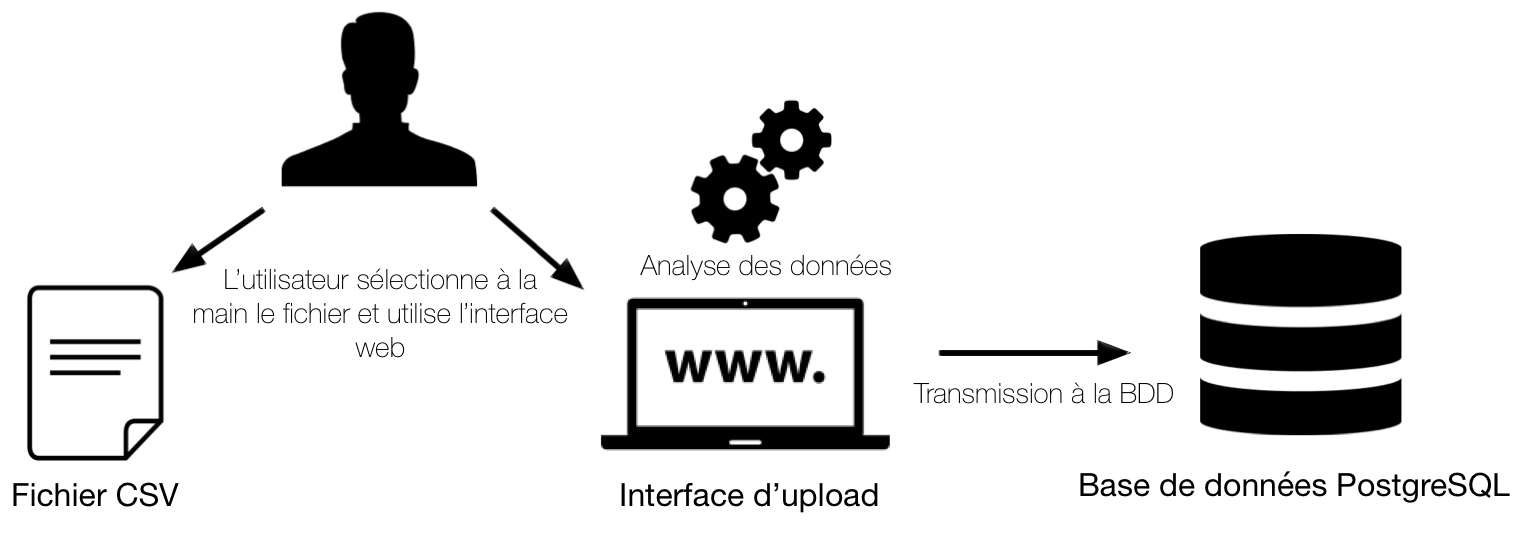
\includegraphics[scale=0.57]{images/datafit.png}
\captionof{figure}{Principe de l'interface d'upload}
\label{interface_upload}
\end{center}


Le diagramme de cas d'utilisation \ref{arena_pricing_use_case} page \pageref{arena_pricing_use_case} détail les différentes possibilités d'envoie de données pour un utilisateur :
\begin{itemize}
	\item[\textbullet] Via un fichier CSV d'export contenant les données billétteries, le client importe envoie ce fichier sur l'interface d'upload du site.
	\item[\textbullet] Via une API, il peut demander directement le "rapatriement" des données 
\end{itemize}


\begin{center}
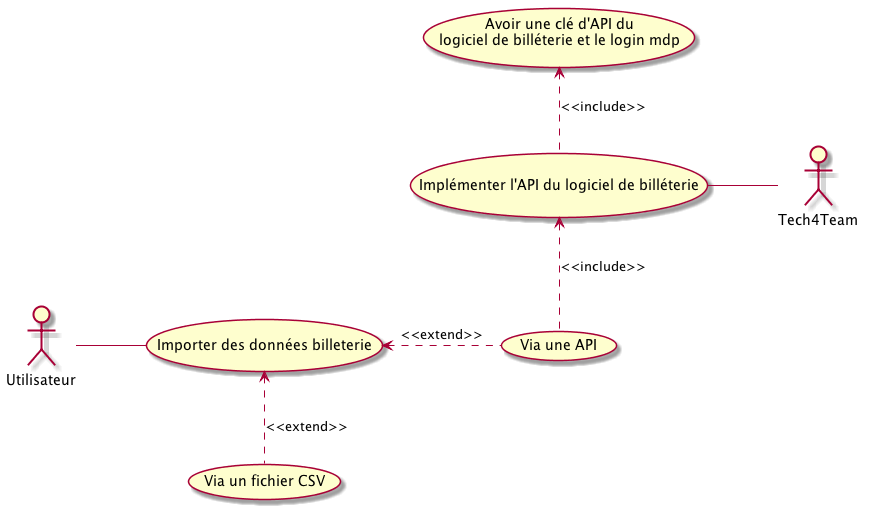
\includegraphics[scale=0.57]{images/arenapricing-use-case.png}
\captionof{figure}{Diagramme de cas d'utilisation de l'interface d'upload d'ArenaPricing}
\label{arena_pricing_use_case}
\end{center}


\subsection{Première réalisation du front d'importation}

Pour réaliser ce site web d'importation nous avons décidé après discussion avec le lead developper d'utiliser le langage Python. Ce langage permet de développer rapidement et dispose de nombreux modules s'ajoutant aux fonctions de base. Il est ainsi aisé de parser un fichier CSV. J'ai également utilisé le microframework Flask pour créer les pages web en elle même et servir de serveur web. Pour le design du site, j'ai utilisé le framework Zurb Foundation afin d'avoir une identité visuelle cohérente avec le reste du site ArenaMetrix. 

\begin{center}
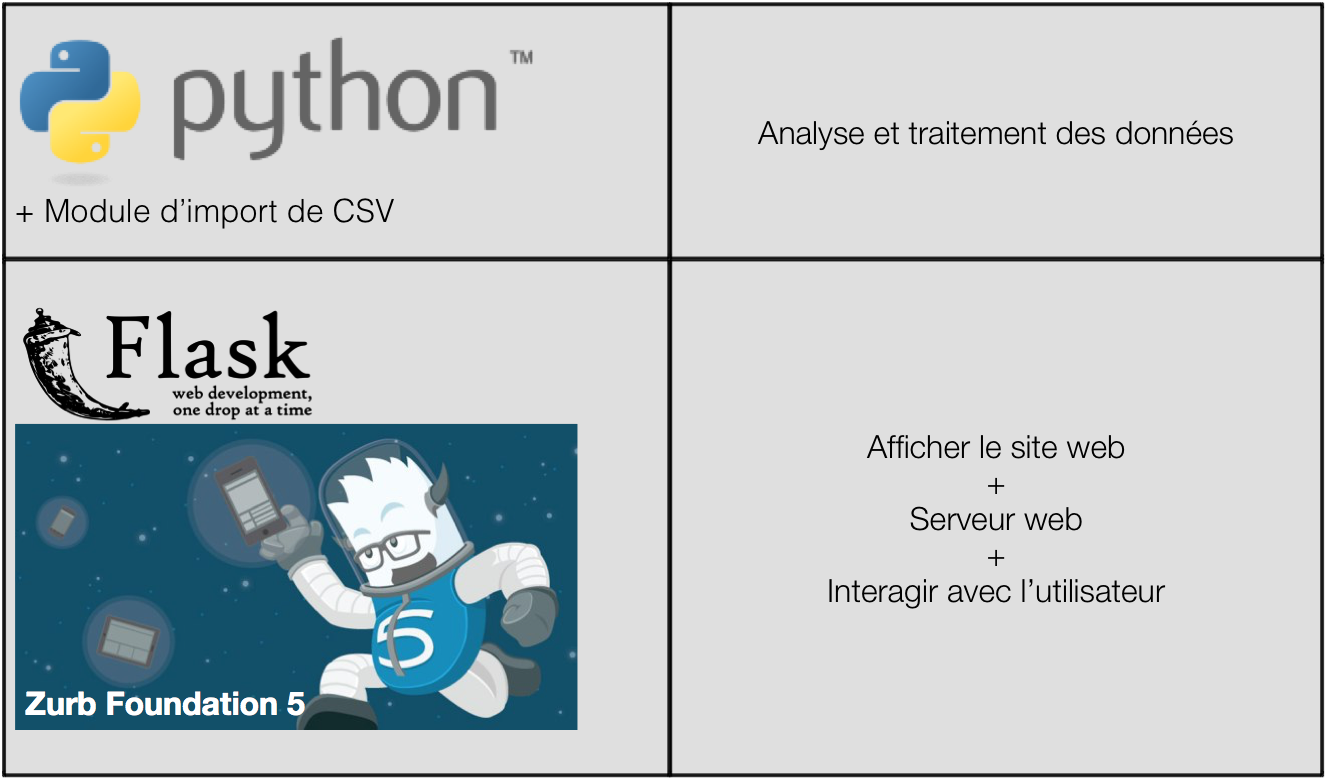
\includegraphics[scale=0.6]{images/datafit2.png}
\captionof{figure}{Téchnologies utilisées pour le front}
\label{interface_upload_tech}
\end{center}

\subsubsection{L'interface homme-machine obtenue}

Comme nous pouvons le voir sur l'impression d'écran \ref{front_upload} page \pageref{front_upload} l'interface permet à l'utilisateur d'envoyer un fichier CSV préalablement sélectionné.
En plus du nom de l'organisation, nous affichons le type d'événement correspondant au fichier envoyé ainsi que le logiciel de billetterie d'où provient l'export. \\

\begin{center}
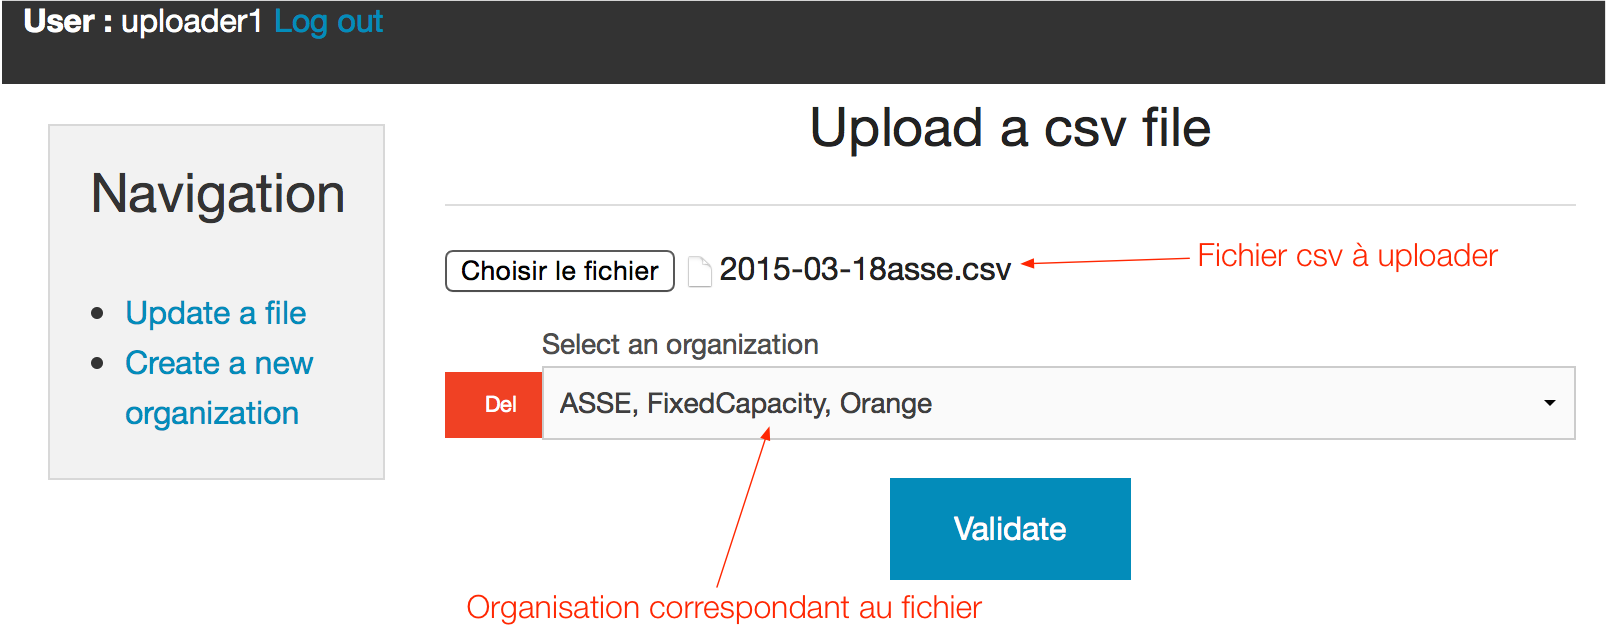
\includegraphics[scale=0.6]{images/front1.png}
\captionof{figure}{Front d'upload d'un fichier CSV}
\label{front_upload}
\end{center}

\subsubsection{Parsing des données en Python}
Pour parser les fichiers CSV j'utilise le module natif CSV. Le principal problème avec les fichier CSV est l'encodage, parfois c'est du UTF-8, d'autres fois du latin1 ou encore du windows-1252. Le module $chardet$ permet de détecter l'encodage d'un fichier.
\\


\lstset{style=custompython}
\begin{lstlisting}
f = open(p_path_file, 'rb')
charset_char = f.read(10000) #read 10000 first characters to detect charset
f.close()
charset = chardet.detect(charset_char)
with open(file_path, 'r', encoding=charset['encoding']) as f:

	#read csv file with csv module
	dict_csv = csv.DictReader(f, delimiter=';', quoting=csv.QUOTE_ALL)
	
	#use strategy design pattern with Secutix object
	secutix = ParsingStrategyContext(Secutix())	
	
	#parse dictionay and send organization name, event date, export date
	secutix.parse_file(dict_csv, o_name, e_date, export_date)

#ask object to send data to the ruby. e_type is event type 
reason = secutix.upload_data(e_type)
return reason
\end{lstlisting}
\captionof{lstlisting}{Code analysant le fichier CSV}

\leavevmode \\
La fonction open permet d'ouvrir le fichier $file\_path$, ensuite je récupère le dictionnaire associé à au fichier CSV avec $csv.DictReader$. La méthode $parse\_file$ permet de générer le dictionnaire avec les informations des tickets/achats comme le montre la figure \ref{dict_csv} page \pageref{dict_csv}, nous obtenons finalement une liste de dictionnaire ou chaque entrée de la liste est une ligne du fichier CSV. 

\begin{center}
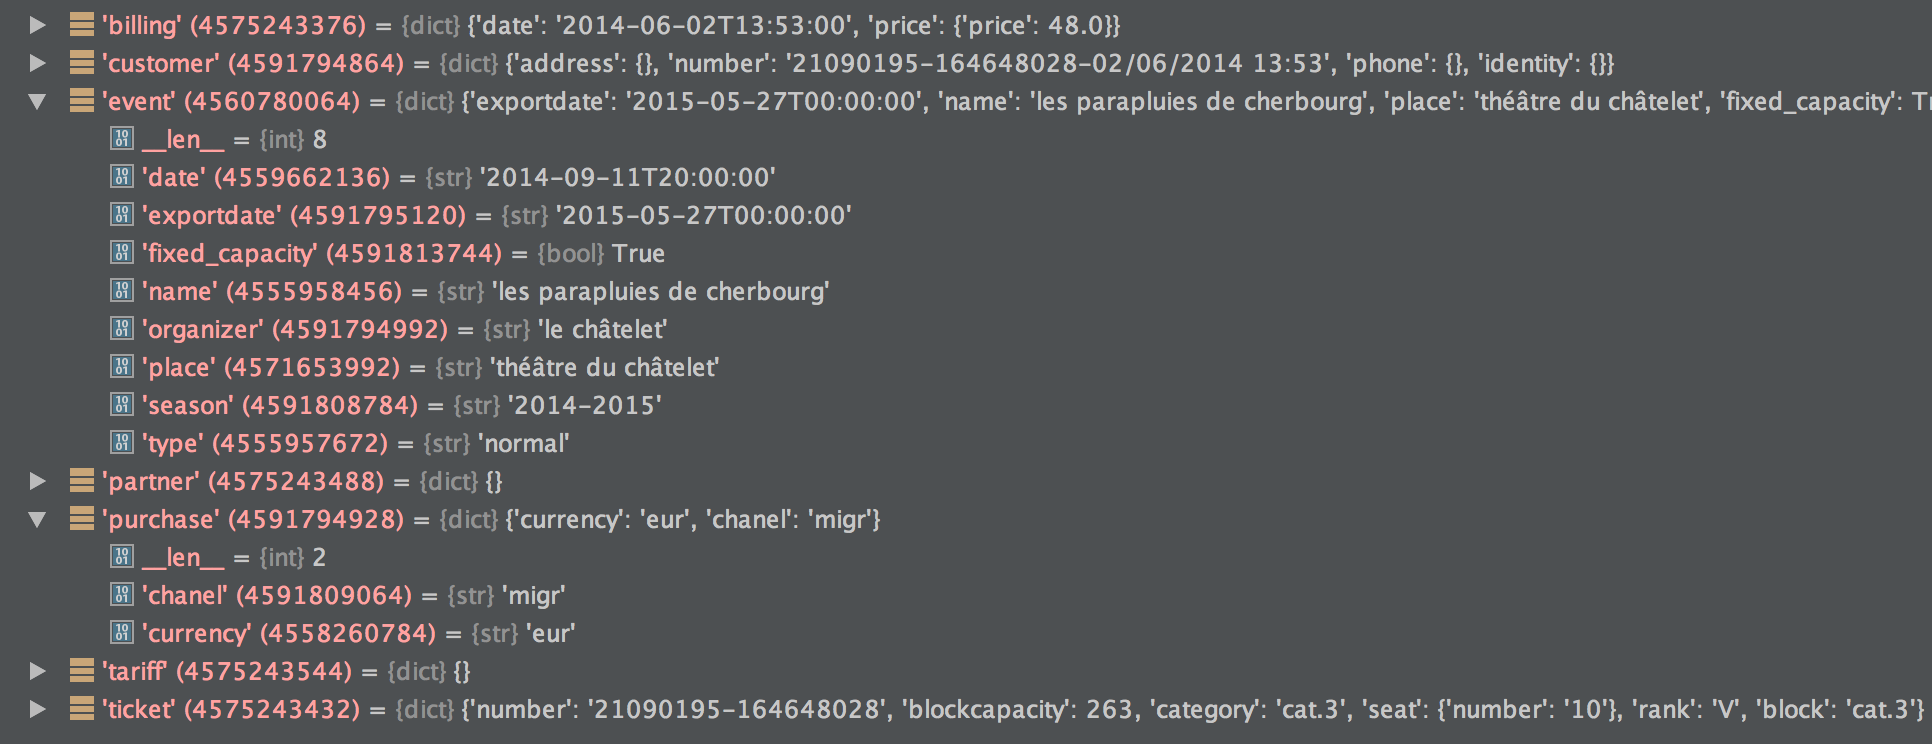
\includegraphics[scale=0.45]{Images/dict_tickets.png}
\captionof{figure}{Dictionnaire récupéré pour une ligne du fichier CSV}
\label{dict_csv}
\end{center}

D'un point de vue architecture de l'application j'utilise le design pattern strategy. Ce design pattern est utile lorsqu'un objet peut effectuer plusieurs traitements différents, dépendant d'une variable ou d'un état.

L'implémentation de ce design pattern peut être visualisé sur le diagramme figure \ref{stategy_pattern} page \pageref{dict_csv}.

\begin{center}
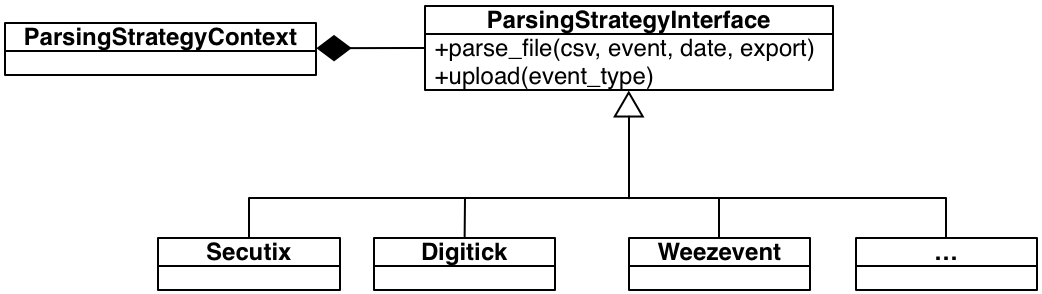
\includegraphics[scale=0.75]{Images/StrategyPattern.png}
\captionof{figure}{Design pattern strategy}
\label{stategy_pattern}
\end{center}


\subsubsection{Problèmatique posée par ce logiciel}
Après avoir testé le logiciel d'importation avec de nombreux clients, il s'avère que les fichiers fournis ne sont pas générique. \\
Les noms des colonnes ne sont pas les mêmes en fonction des exports alors que le logiciel de billetterie est identique et dans certains cas le changement apparait pour un même client d'une saison à l'autre. \\
On se rend donc rapidement compte que nous ne pouvons pas créer un script unique par logiciel de billetterie.
\\

La partie front en Flask n'est actuellement plus utilisée, mais le python qui permet de parser les données et utilisé pour les clients qui n'ont pas d'API et qui uploadent donc des fichiers CSV sur un serveur FTP. 


\subsection{Deuxième itération pour le logiciel d'import des fichiers}
Nous décidons de repenser notre logiciel pour que le client désirant envoyer un fichier CSV puisse spécifier sur l'interface les champs qu'il souhaite importer.

Comme le montre l'image \ref{draft_front_import2} page \pageref{draft_front_import2} du premier draft que j'ai réalisé, le client doit maintenant faire un travail d'association entre les champs présents dans le fichier CSV leur correspondance réelle. 

\begin{center}
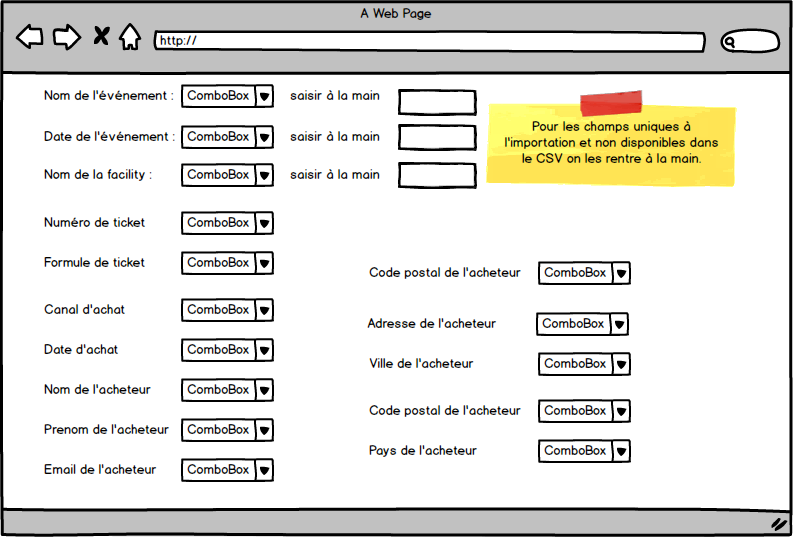
\includegraphics[scale=0.55]{images/front3.png}
\captionof{figure}{Premier draft du logiciel d'importation 2.0}
\label{draft_front_import2}
\end{center}


\subsubsection{Création de l'IHM}
Pour réaliser l'interface d'upload j'ai utilisé le framework Ruby On Rails afin de pouvoir intégrer facilement et directment la page d'upload au reste du site. Après réflexion, il est plus simple pour nous de maintenir le logiciel principal avec une seule et même technologie : le Ruby. Le Python n'est actuellement utilisé que pour les scripts.

\begin{center}
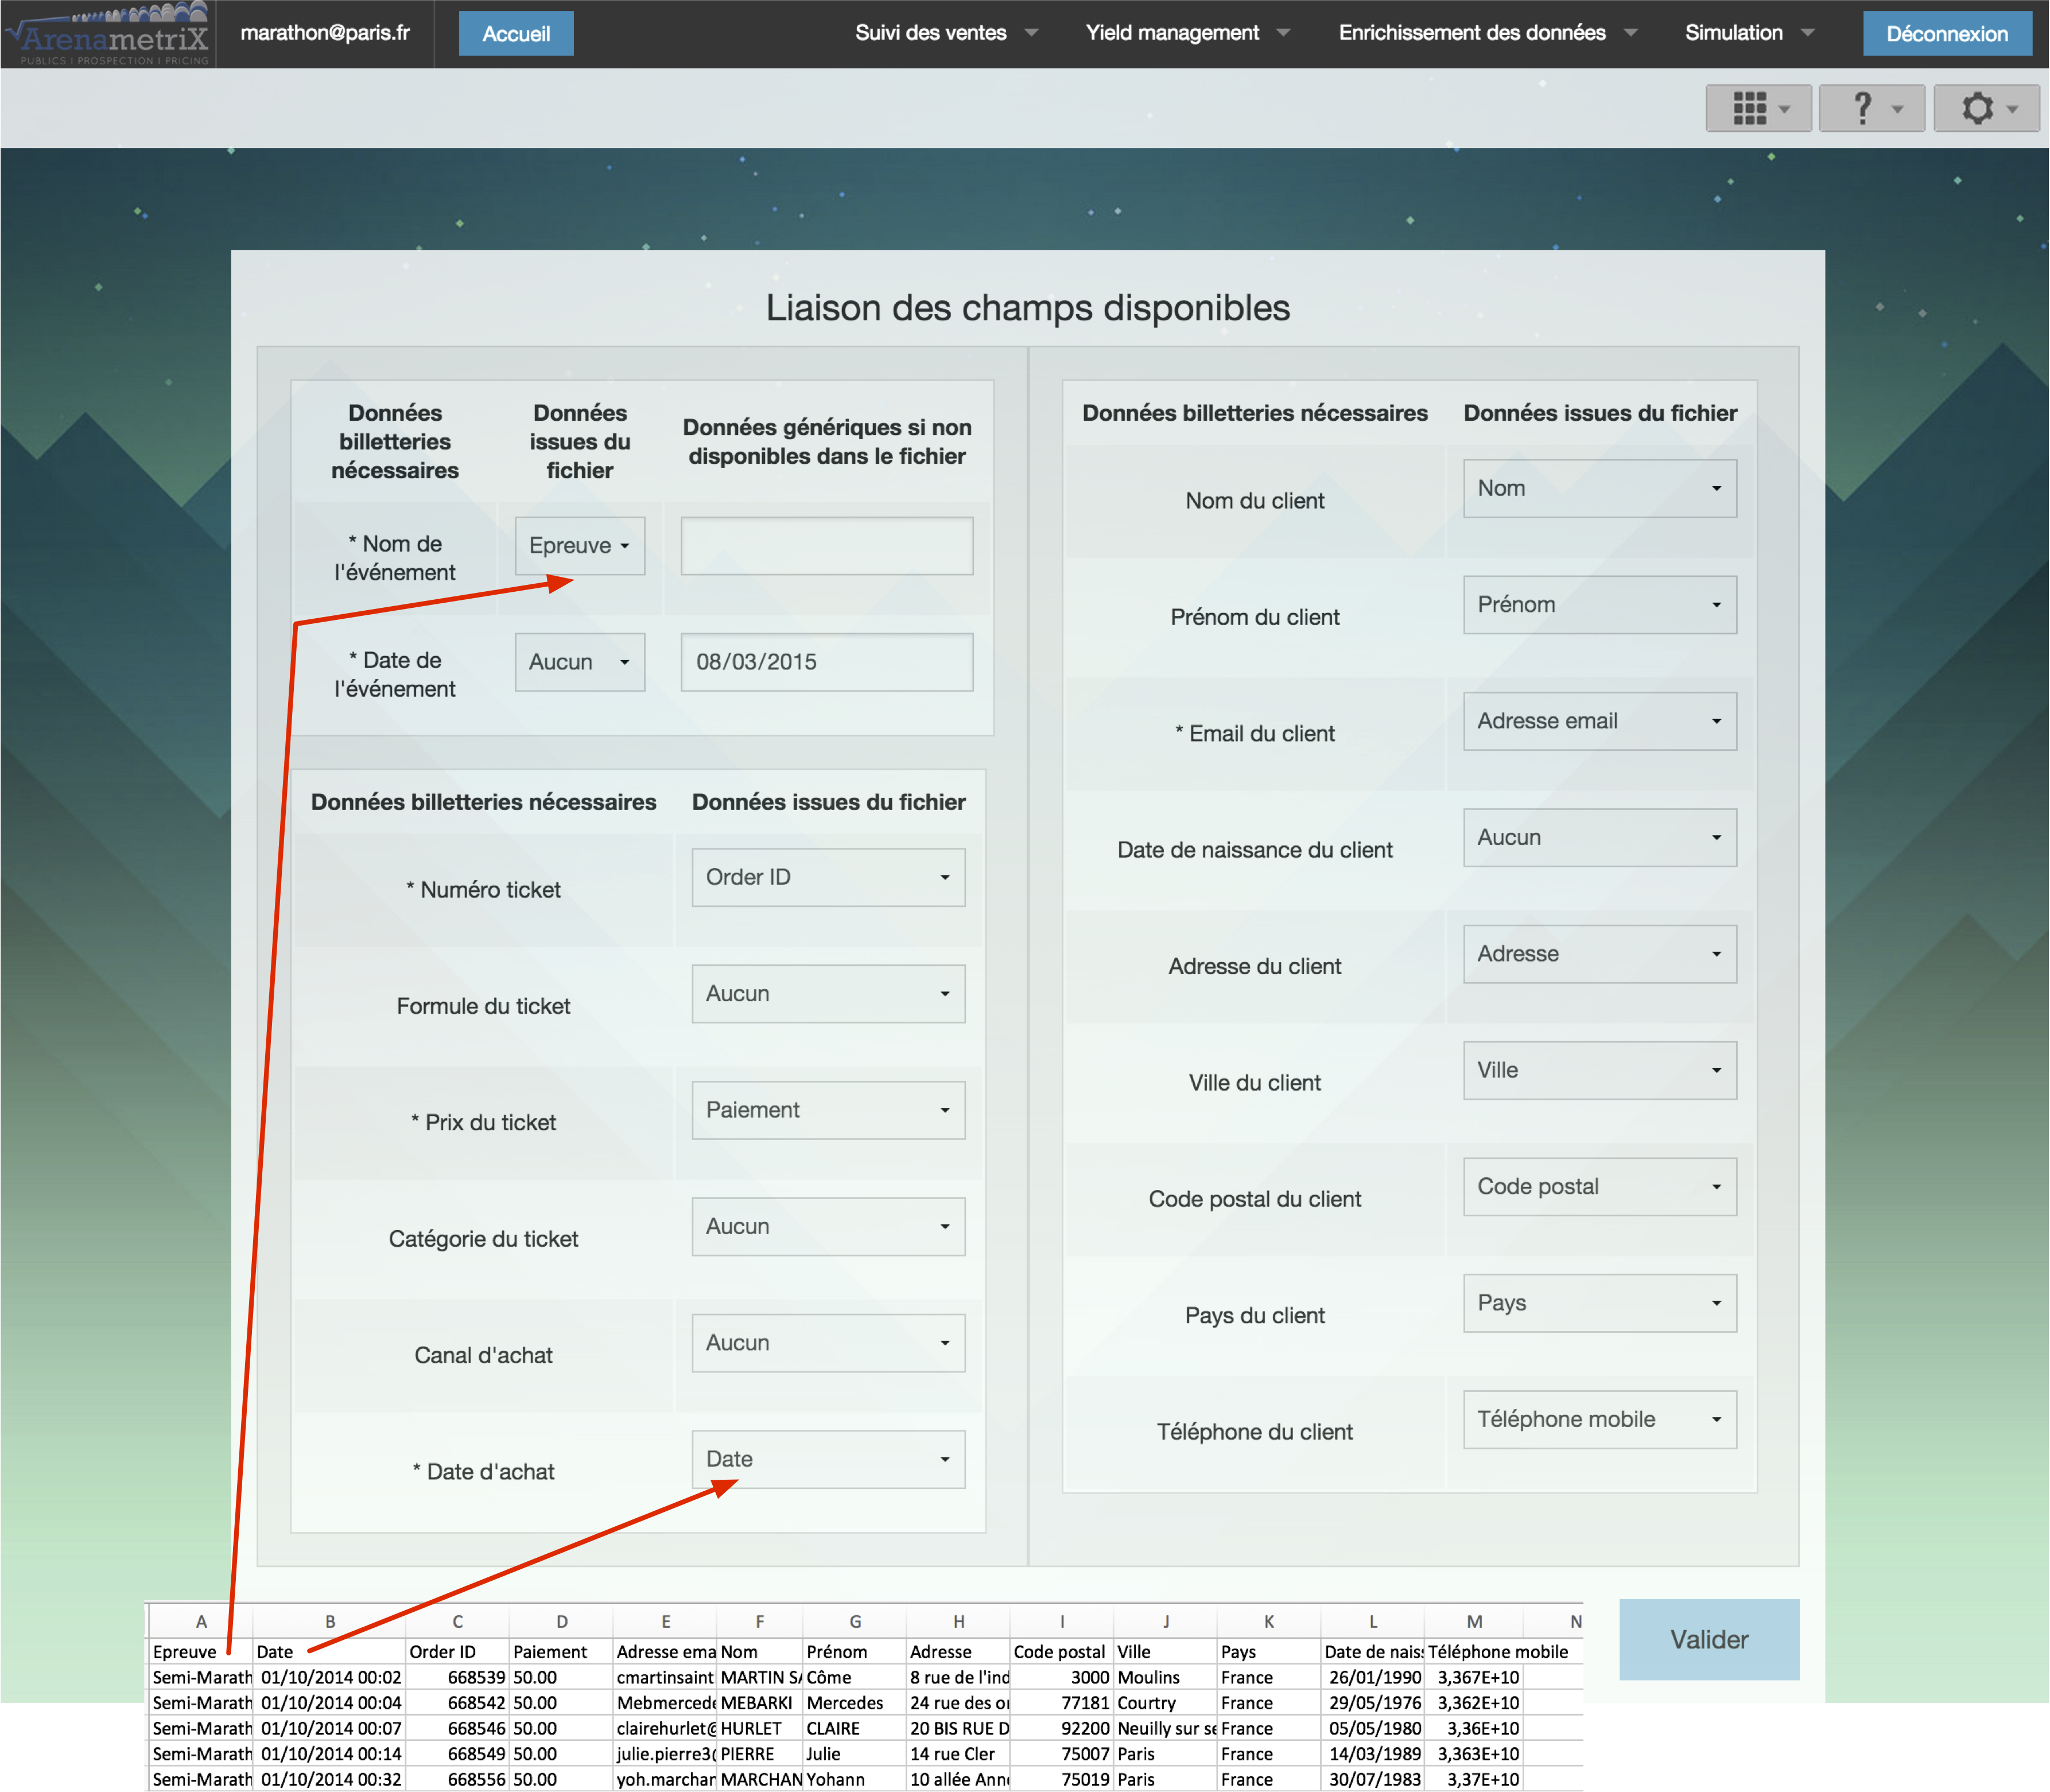
\includegraphics[scale=0.37]{images/final_front2.png}
\captionof{figure}{Logiciel d'importation des clients}
\label{final_front_import2}
\end{center}

J'obtiens finalement le front-end \ref{final_front_import2} page \pageref{final_front_import2}, comme nous pouvons le voir avec le fichier CSV de test les champs sont mappés ensemble. Si la donnée n'est pas présente, une insertion vide se fait en base de données. Les champs marqués avec une étoile sont indispensables. Certains champs si ils sont uniques à l'import, comme le nom de l'événement et la date peuvent être inscrits à la main s’ils ne sont pas fournis dans le fichier CSV.


\subsubsection{L'importation des fichiers CSV}

Afin d'importer les données dans le logiciel de billetterie j'utilise l'ORM ActiveRecord.

\lstset{style=customruby}
\begin{lstlisting}
begin
  country = Pricing::Country.find_by!(name: customer_country_to_ins)
rescue ActiveRecord::RecordNotFound 
  country = Pricing::Country.new(name: customer_country_to_ins)
end
country.save
begin
  department = Pricing::Department.find_by!(name: customer_zip_to_ins, country: country)
rescue ActiveRecord::RecordNotFound
  department = Pricing::Department.new(name: customer_zip_to_ins,  country: country)
end
department.save
begin
  city = Pricing::City.find_by!(name: customer_city_to_ins, department: department)
rescue ActiveRecord::RecordNotFound
  city = Pricing::City.new(name: customer_city_to_ins,  department: department)
end
city.save
\end{lstlisting}
\captionof{lstlisting}{Exemple de code insérant une adresse}
\leavevmode \

Avant d'insérer une donnée, je vérifie si elle est présente, si ce n'est pas le cas je rescue l'exception et j'insère la donnée. 
L'ORM ActiveRecord permet de s'astreindre des contraintes habituelles du SQL, lorsque je fais $coutry: country$ lors d'une intention de département l'ORM comprend qu'il doit lier $country$ comme clé étrangère de $département$.

\subsection{Les API des logiciels billetteries}
Différentes approches pour importer les données sont possibles : 
\begin{itemize}
  \item[\textbullet] Le client nous donne le login et mot de passe de son logiciel billetterie : nous faisons l'extraction d'un fichier CSV et nous l'importons à la main dans la base de données. 
  \item[\textbullet] Le client envoie son fichier CSV par mail : nous l'importons à la main dans la base de données (et lui redemandons le fichier si il manque des champs...).
  \item[\textbullet] Le client dépose son fichier CSV sur un serveur FTP : un script Python est chargé de régulièrement scanner ce serveur FTP et d'importer les données s'il a un changement.
  \item[\textbullet] La société logiciel billetterie nous donne une clé d'API, ainsi avec le mot de passe et login du client nous pouvons accéder aux données en nous connectant directement à la base de données. C'est l'idéal pour nous, cela nous permet d'automatiser les imports.
\end{itemize}

Actuellement nous avons accès aux API des billetteries WeezEvent, Njuko et Digitick. 
Pour récupérer les données des API j'utilise le module request qui permet de faire des requêtes get.
\\ \\
Ainsi la requête suivante me permet de récupérer les événements d'une organisation :

\lstset{style=custompython}
\begin{lstlisting}
json_events = requests.get("https://api.weezevent.com/events",
                            params={'api_key': API_KEY,
                                    'access_token': token,
                                    'include_closed': True}
                          )
events = json_events.json()['events']
for event in events :
	#Traitemet
\end{lstlisting}
\captionof{lstlisting}{Récupération des événements sur l'API de weezevent}
\leavevmode \

À la fin de mon stage, nous avions accès a trois API de logiciel de billetteries : 
\begin{itemize}
  \item[\textbullet] WeezEvent pour les événements :
  \begin{itemize}
	\item Mondial du tatouage : un salon annuel pour les tatoueurs du monde entier
	\item File7 : Une salle de concert en région parisienne. 
	\item Rhum Fest : Un événement et une exposition sur le thème de rhum
  \end{itemize}
  \item[\textbullet] Njuko pour les événements :
  \begin{itemize}
  	\item Marathon de Paris
  \end{itemize}
  \item[\textbullet] Digitick pour :
  \begin{itemize}
  	\item Le musée Grévin
  \end{itemize}

\end{itemize}

\subsection{La base de données en elle même}
L'architecture de la base de données ArenaPricing peut être visualisée sur la figure \ref{arenapublic-1} de l'annexe page \pageref{arenapublic-1}.
\\

Cette base de données de la première forme normale car tous ses attributs de la base de données ont des valeurs simples (non multiples, non composées).
\\

Elle est également en deuxième forme normale car aucun attribut non clé ne dépend d'une partie de la clé.
\\

Et de troisième forme normale car aucun attribut non clé ne dépend d'un ou plusieurs attributs ne participant pas à la clé.



%TODO Parler des formes normales

		


\end{document}